\subsection{Subversion Branches and Tags}
\label{section_branches_and_tags}
\renewcommand{\figurename}{Diagram}

Creation, deletion or replacement of any of the Subversion /branches/\emph{branch} or /tags/\emph{tag} directory
is translated into creation, deletion or replacement of the corresponding Git reference object (Git tag or branch). 
\\\\
Depending on the absence or presence of the actual contents modification accompanying creation of the /branches/\emph{branch} 
or /tags/\emph{tag} directory, translation may or may not result in a Git commit creation, additionally 
to the reference object creation.
\\\\
There is no technically enforced difference between Subversion branches and tags. Translator, however, translates
/branches/\emph{branch} directories into Git branch references and /tags/\emph{tag} directories into Git tag objects.
Thus there are no differences in translation of Subversion branches and tags, except for those outlined below:
\begin{enumerate}
	\compactlist
	\item On creation
	\begin{itemize}
		\item Creation of /branches/\emph{B} directory leads to creation of a new branch reference \emph{B}.
		\item Creation of /tags/\emph{T} directory leads to addition of corresponding Tag Object with name \emph{T}.
	\end{itemize}
	\item On modification
	\begin{itemize}
		\item Modification which affects paths in /branches/\emph{B} directory leads to updating of corresponding branch reference \emph{B}.
		\item Modification which affects paths in /tags/\emph{T} directory leads to the removal of obsolete Tag Object with name \emph{T} and creation of new Tag Object with the same name \emph{T} for corresponding Commit Object.
	\end{itemize}
	\item On removal
	\begin{itemize}
		\item Removal of /branches/\emph{B} directory leads to removal of corresponding reference \emph{B} at Git repository, when
		\item Removal of /tags/\emph{T} directory leads to removal of corresponding Tag Object with name \emph{T}.
	\end{itemize}
\end{enumerate}
Further scenarios specifies translation rules for Subversion branches, but are applicable for Subversion tags as well, 
with the differences outlined above being taken into account.
%\\\\
%The same rules could be treated in opposite direction --- every change of Git branch or tag leads to corresponding change of Subversion branch or tag.
%\\\\
%This and further chapters consider scenarios with branches only. Every scenario could be applied to tags with the rules above taken into account.
%\\\\
%Basically Translator tracks all the references located at Git repository and synchronizes every such reference with certain Subversion branch. The exact way of this synchronization described further.

\subsubsection{Subversion Branch Creation}

For the purpose of this specification, Subversion branch is a subdirectory in the top-level /branches directory of
Subversion repository. Name of that very subdirectory is a branch name. /trunk top-level directory is considered to be a branch named \emph{master}.
/trunk branch always exists in Subversion repository. Other branches might be created in different ways and thus there are 
multiple ways to translate branch creation.
\\\\
1. Most common way to create a Subversion branch is to make a copy of another branch at particular revision.
Diagram \ref{branch_creation_svn_to_git} depicts translation of a new Subversion branch \emph{/branhces/branch2} created 
at revision r3 into creation of a Git commit \emph{c} and creation of a Git branch reference \emph{branch2}. Relationship 
between \emph{/branches/branch2} and \emph{/branches/branch1} is translated into a child-parent reference between new commit \emph{c} and commit \emph{b}.
\begin{center}
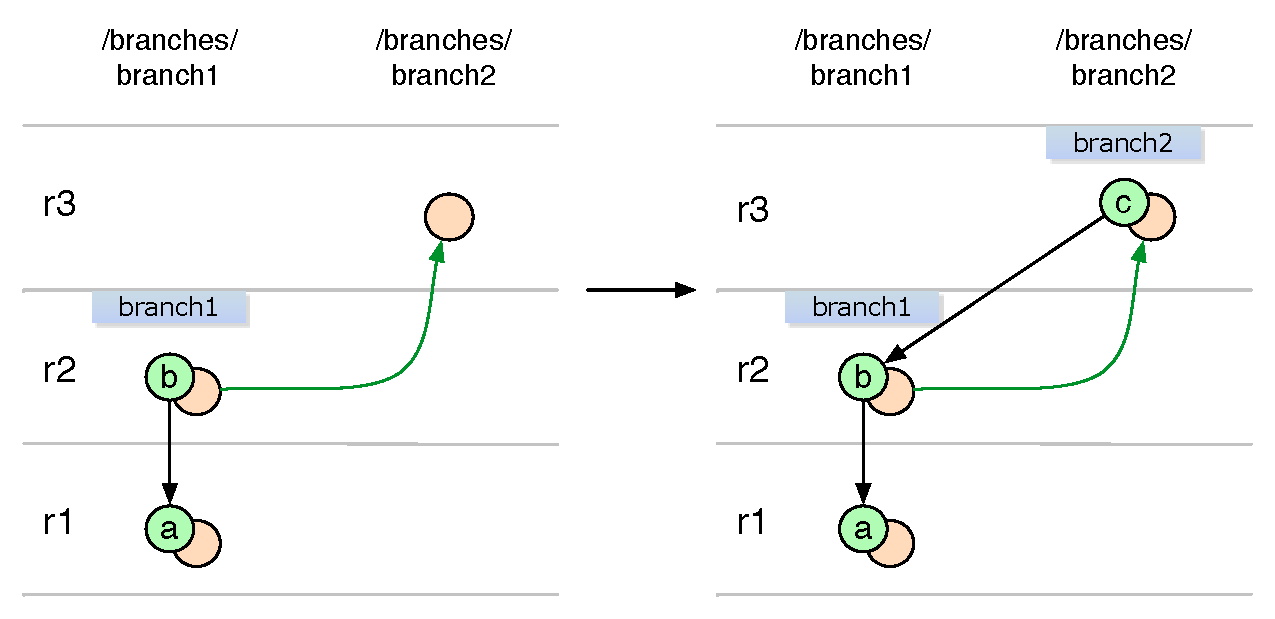
\includegraphics[width=\textwidth]{img/diagrams/branch_creation_svn_to_git.pdf}%
\captionof{figure}{Subversion branch copy being translated to Git branch creation.}
\label{branch_creation_svn_to_git}%
\end{center}
New Git commit \emph{c} contents might or might not be different from that of the Git commit \emph{b}. 
This depends on whether Subversion branch creation included content modification or not. New Git commit
\emph{c} preserves metadata of Subversion revision 3, in particular author, commit message and commit date.
\\\\
2. Another, less common way to create a branch in Subversion is to create new directory in /branches top-level
folder and then merge changes made on another branch into the newly created directory. This way
establishes relationship between new and original branch with the help of merge tracking information.
\\\\
Diagram \ref{branch_creation_from_mergeinfo_svn_to_git} demonstrates how this kind of branch origin 
is translated into the child-parent reference between new and previous commit, just like in the 
case of branch created by copying.
\begin{center}
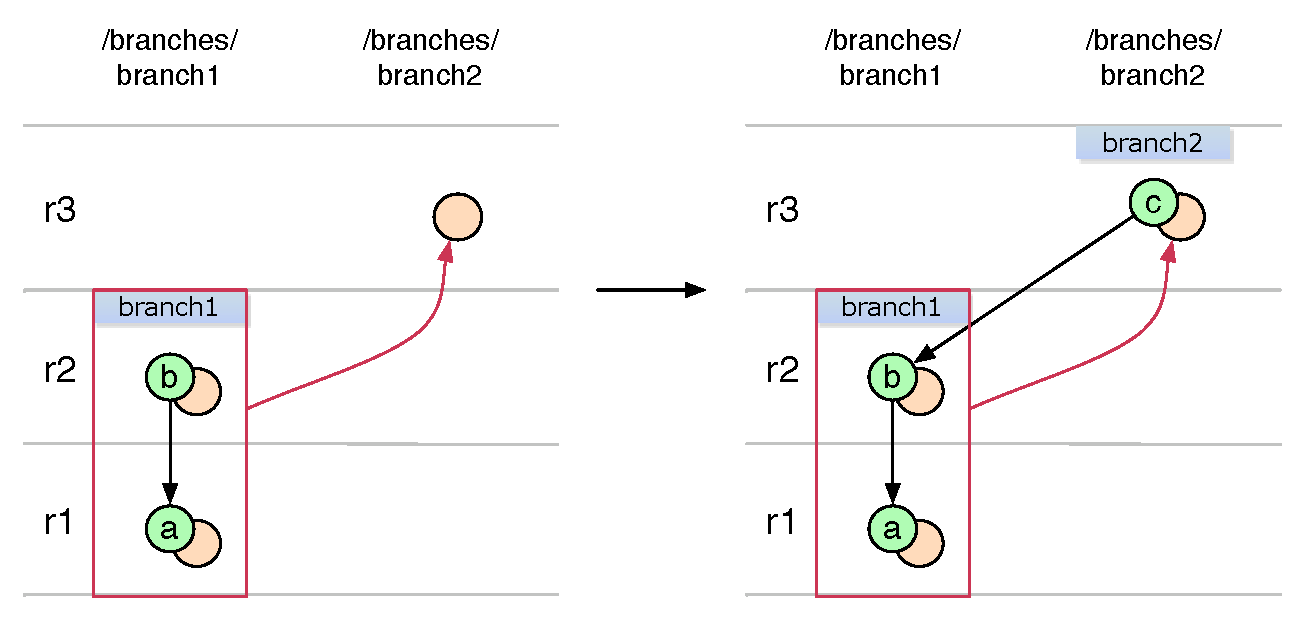
\includegraphics[width=\textwidth]{img/diagrams/branch_creation_from_mergeinfo_svn_to_git.pdf}%
\captionof{figure}{Subversion branch addition with merge history being translated to Git branch creation.}
\label{branch_creation_from_mergeinfo_svn_to_git}%
\end{center}

3. Finally, branch might be created with empty history, i.e. with no reference to any of the existing 
revisions. In this case, as shown on the diagram \ref{branch_creation_no_history_svn_to_git} no child-parent
reference is created for the new Git commit \emph{c}. % vs: Initial revision of the whole repository is translated in the same manner.

\begin{center}
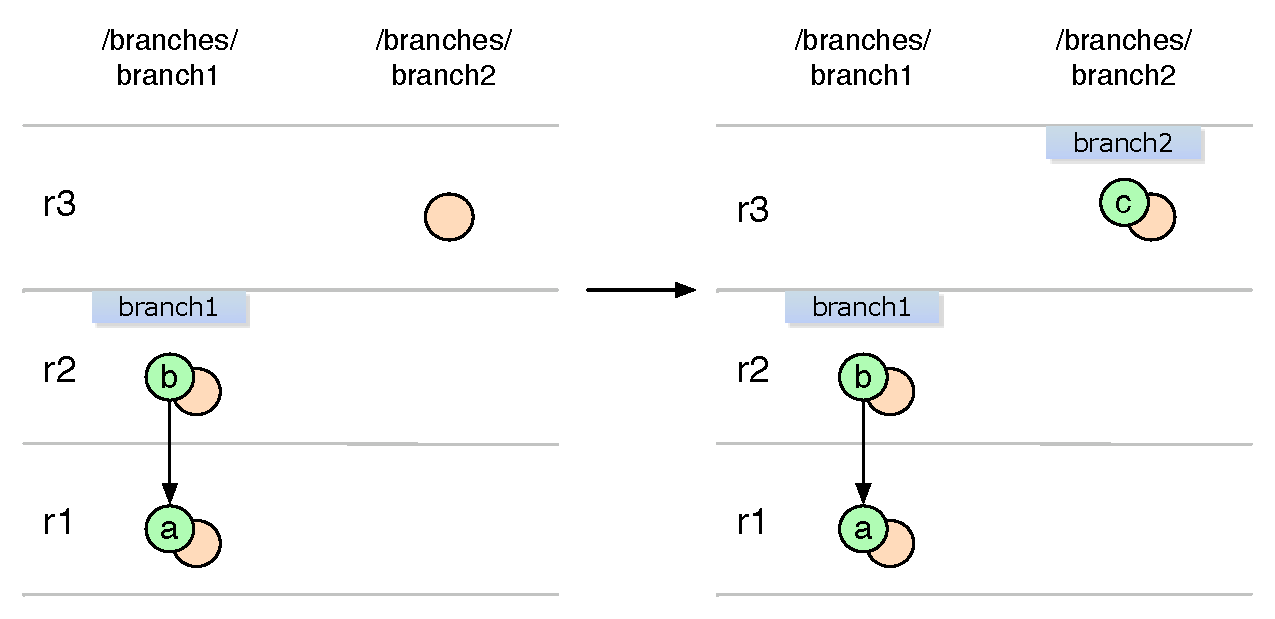
\includegraphics[width=\textwidth]{img/diagrams/branch_creation_no_history_svn_to_git.pdf}%
\captionof{figure}{Subversion branch addition with no history being translated to creation of Git branch referenced to commit with no parents.}
\label{branch_creation_no_history_svn_to_git}%
\end{center}

\subsubsection{Modification on Subversion Branch}

As already specified in the previous section (see \ref{section_revisions_and_commits}), Subversion
revision is translated into multiple Git commits - one Git commit for each group of 
affected paths, paths being grouped by the branch they belong to.
\\\\
See diagram \ref{double_branch_change_svn_to_git} for an example of multiple commits 
on different Git branches being created for a single Subversion revision.

\begin{center}
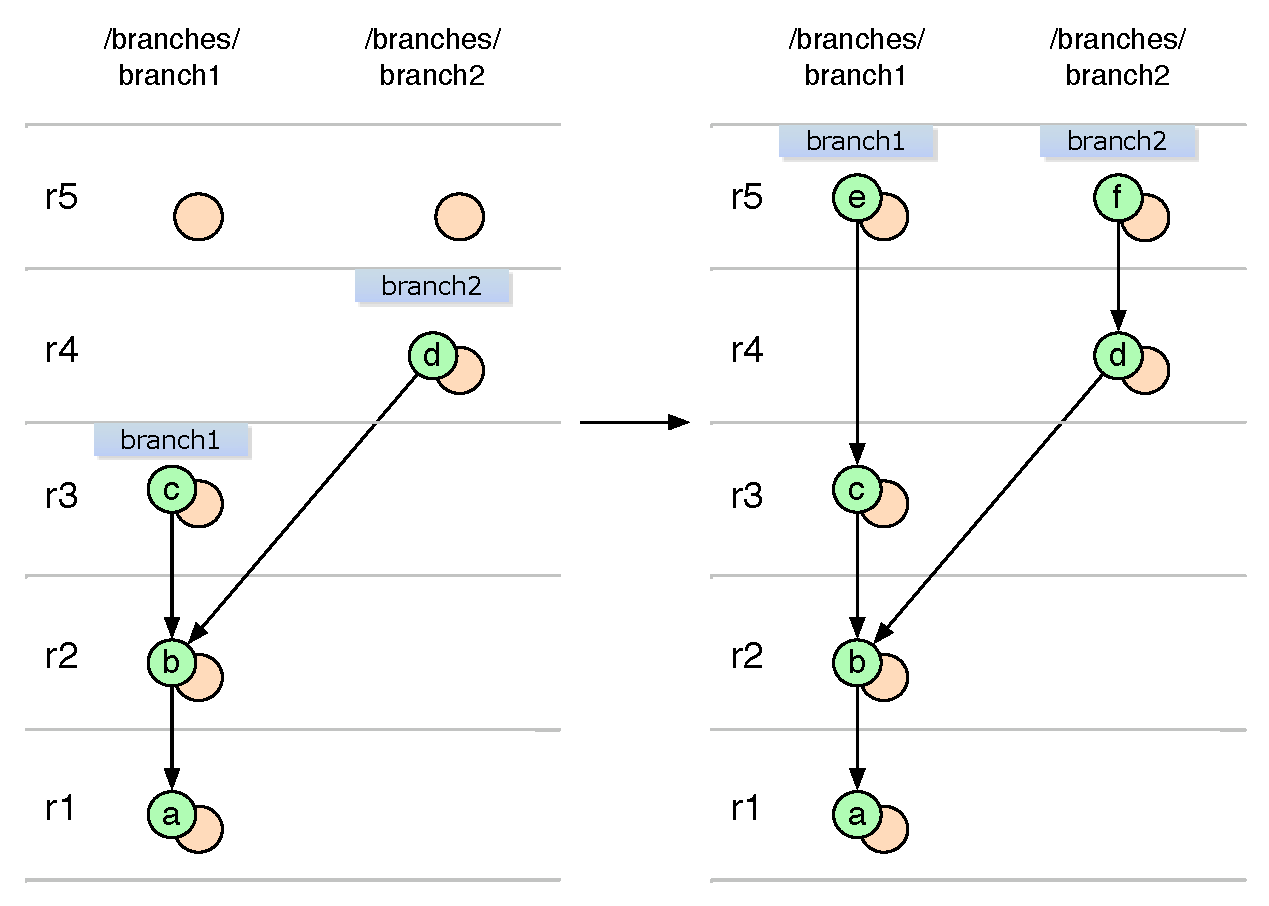
\includegraphics[width=\textwidth]{img/diagrams/double_branch_change_svn_to_git.pdf}%
\captionof{figure}{Revision modified two branches at once being translated to creation of two commits and updating corresponding branch references.}
\label{double_branch_change_svn_to_git}%
\end{center}

\subsubsection{Deletion of Subversion Branch}

Deletion of Subversion branch is always translated into deletion of the corresponding Git branch reference
as shown on the diagram \ref{branch_deletion_svn_to_git}. Single Subversion revision might delete an arbitrary number of branches, 
and thus result in multiple branch references being deleted in Git repository on translation.
\begin{center}
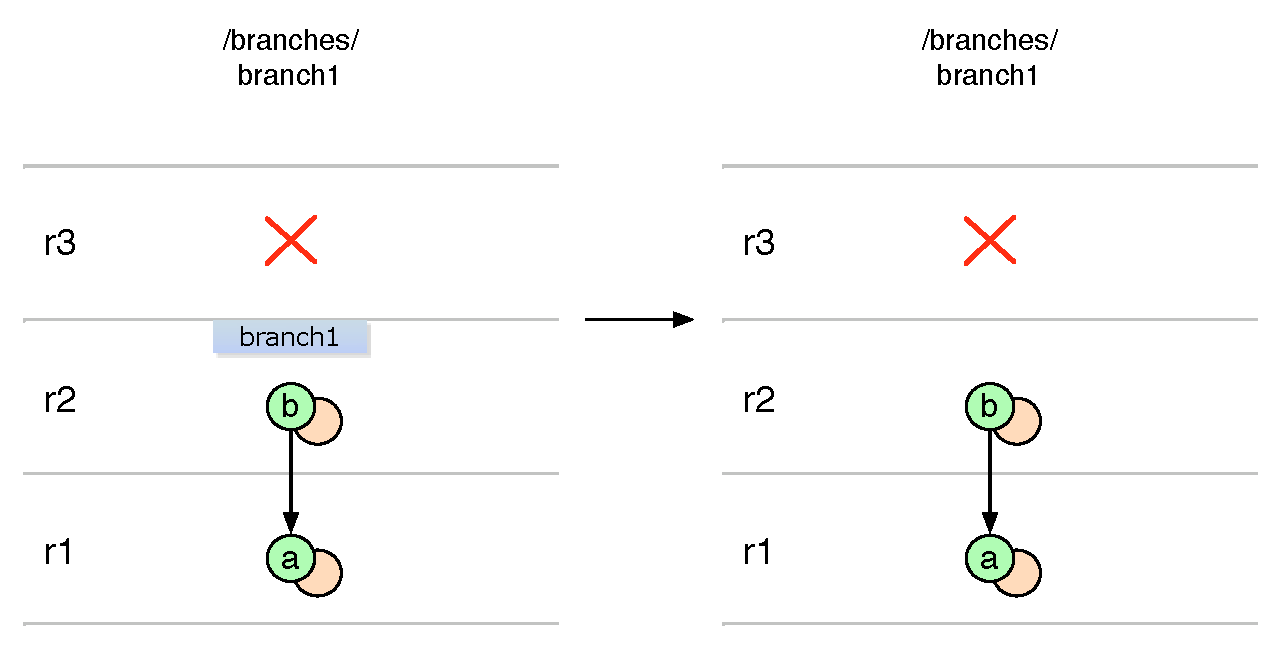
\includegraphics[width=\textwidth]{img/diagrams/branch_deletion_svn_to_git.pdf}%
\captionof{figure}{Deletion of Subversion branch being translated to Git branch removal.}
\label{branch_deletion_svn_to_git}%
\end{center}

\subsubsection{Replacement of Subversion Branch}

Subversion user is able to replace once branch by another with the same name. % vs: "once" or "one"?
Translation of that special case is performed as shown on diagram \ref{branch_replacement_svn_to_git}.
\begin{center}
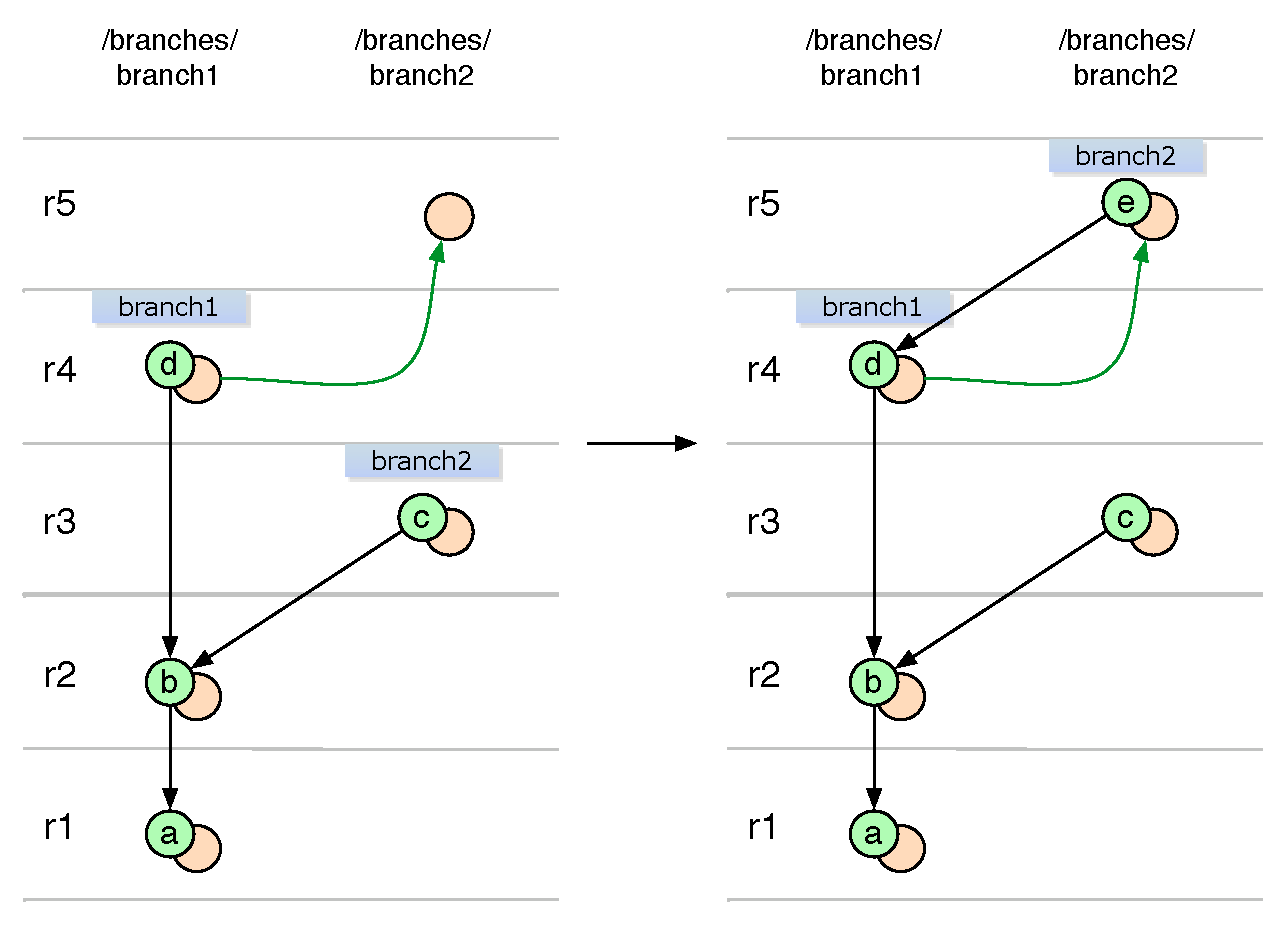
\includegraphics[width=\textwidth]{img/diagrams/branch_replacement_svn_to_git.pdf}%
\captionof{figure}{Replacement of Subversion branch being translated to replacement of Git branch.}
\label{branch_replacement_svn_to_git}%
\end{center}

\subsection{Git Branches and Tags}

To translate Git branches and tags into corresponding Subversion entities, Translator
constantly tracks current set of the reference objects in the Git repository. Whenever % vs: reference objects are here again. Maybe references to commit objects? I don't what is better.
Translator discovers that there is new, modified or deleted reference objects in the Git 
repository, it creates, modifies or deletes corresponding directory in the Subversion repository.
\subsubsection{New Git Branch}

New Git branch reference discovered might refer to the new, not yet translated Git commit object
which has parent commit (diagram \ref{branch_creation_git_to_svn}), to the new Git commit without
reference to a parent commit (diagram \ref{branch_creation_no_history_git_to_svn}) or to the 
existing Git commit (diagram \ref{svn_no_change_branch_creation_git_to_svn}).

\begin{center}
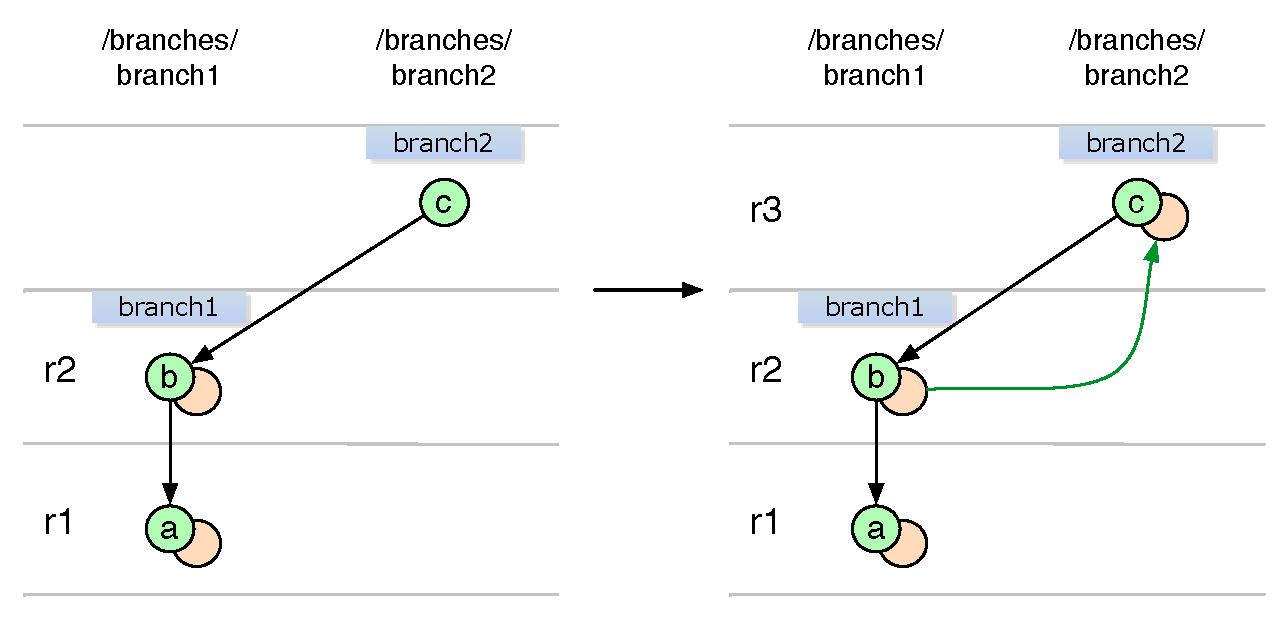
\includegraphics[width=\textwidth]{img/diagrams/branch_creation_git_to_svn.pdf}%
\captionof{figure}{Git branch addition being translated to Subversion branch copy.}
\label{branch_creation_git_to_svn}%
\end{center}

\begin{center}
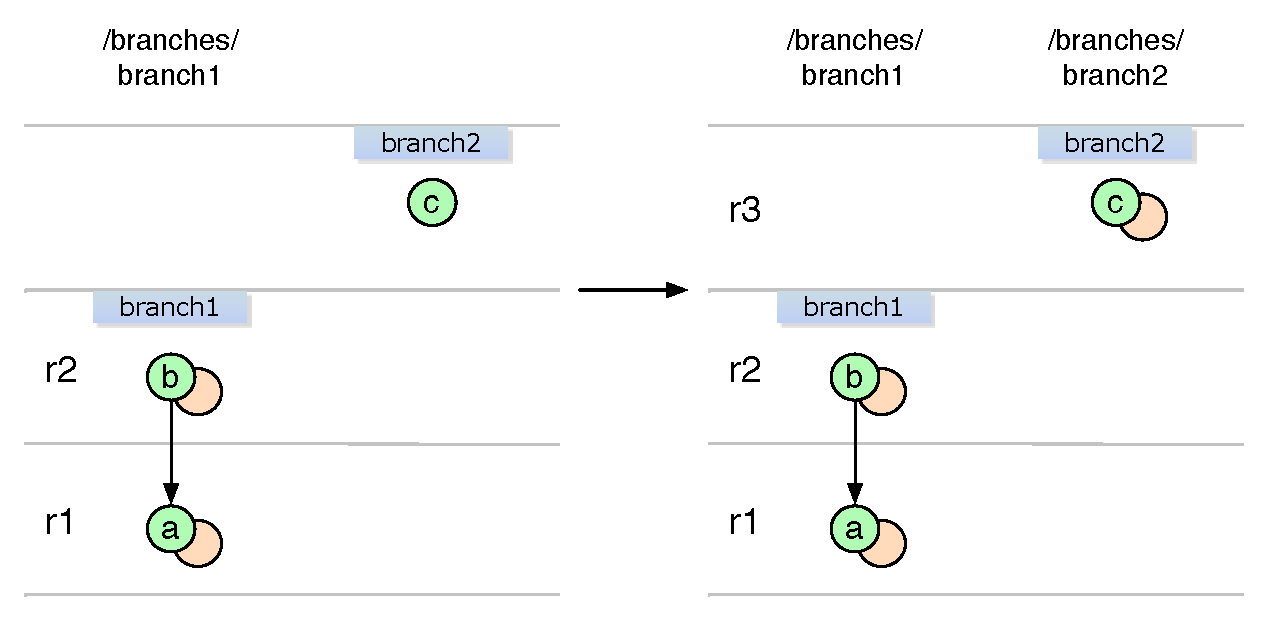
\includegraphics[width=\textwidth]{img/diagrams/branch_creation_no_history_git_to_svn.pdf}%
\captionof{figure}{Addition of Git branch referenced to commit with no parents being translated to Subversion branch creation.}
\label{branch_creation_no_history_git_to_svn}%
\end{center}

\begin{center}
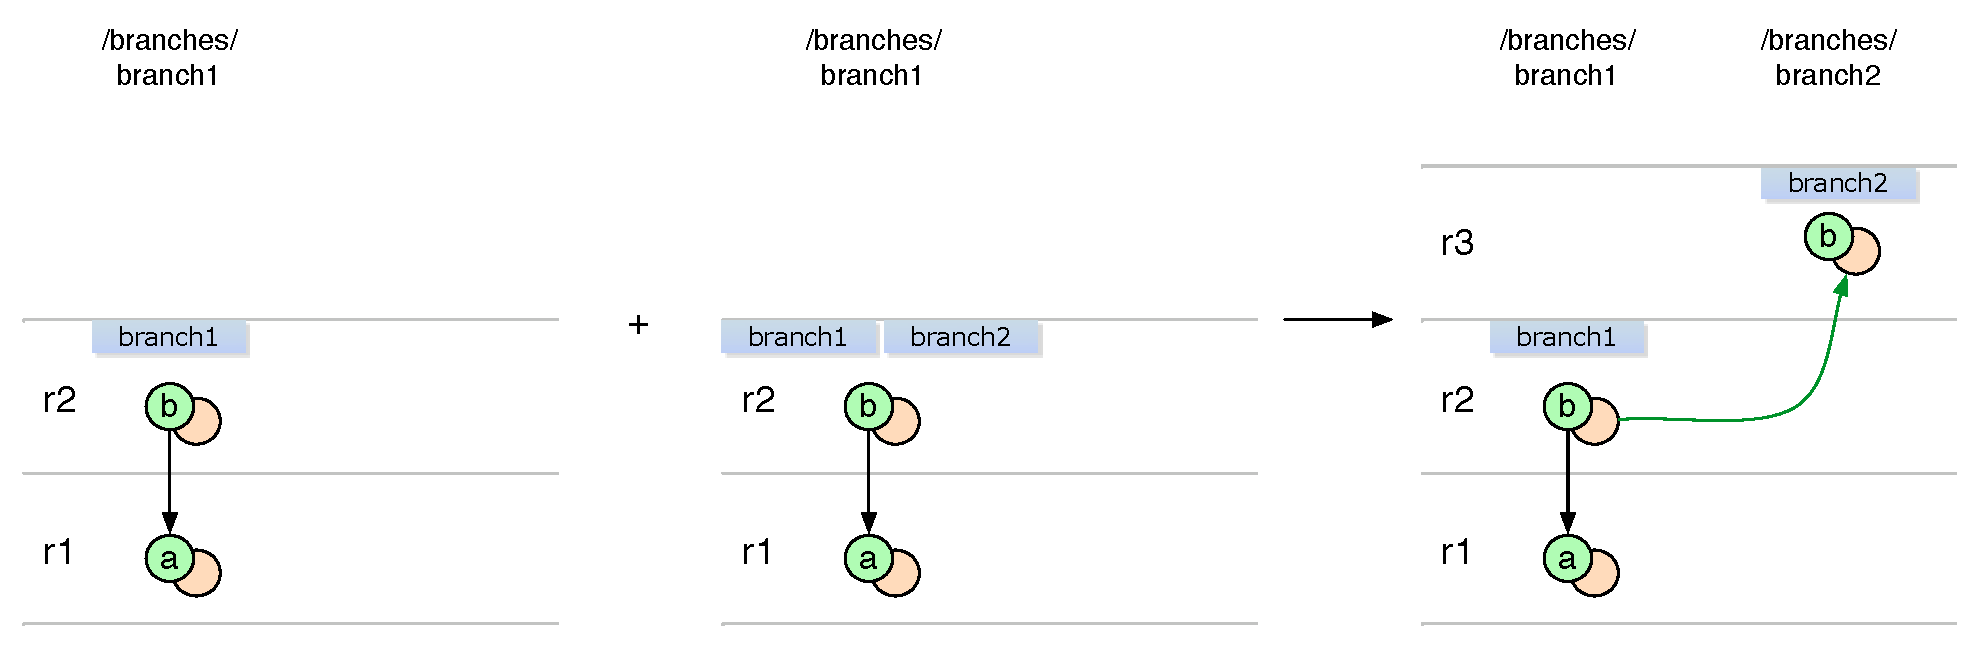
\includegraphics[width=\textwidth]{img/diagrams/svn_no_change_branch_creation_git_to_svn.pdf}%
\captionof{figure}{Addition of second reference to Git commit being translated to creation of Subversion branch with no changes.}
\label{svn_no_change_branch_creation_git_to_svn}%
\end{center}

In the last case, Subversion revision r3 is synthetic, with automatically generated commit message and commit date of the time
revision was created.
\\\\
Combination of the new Git commits on existing branch and new Git branch reference pointing to the latest commit,
is also translated into a new Subversion branch creation, as shown on the diagram \ref{ambiguous_svn_branch_git_to_svn}.
All the new Git commits are translated to the modifications of the first branch, and then as many new branches 
are copied from this first branch as there are new branch references pointing to the latest Git commit on the 
first branch.
\begin{center}
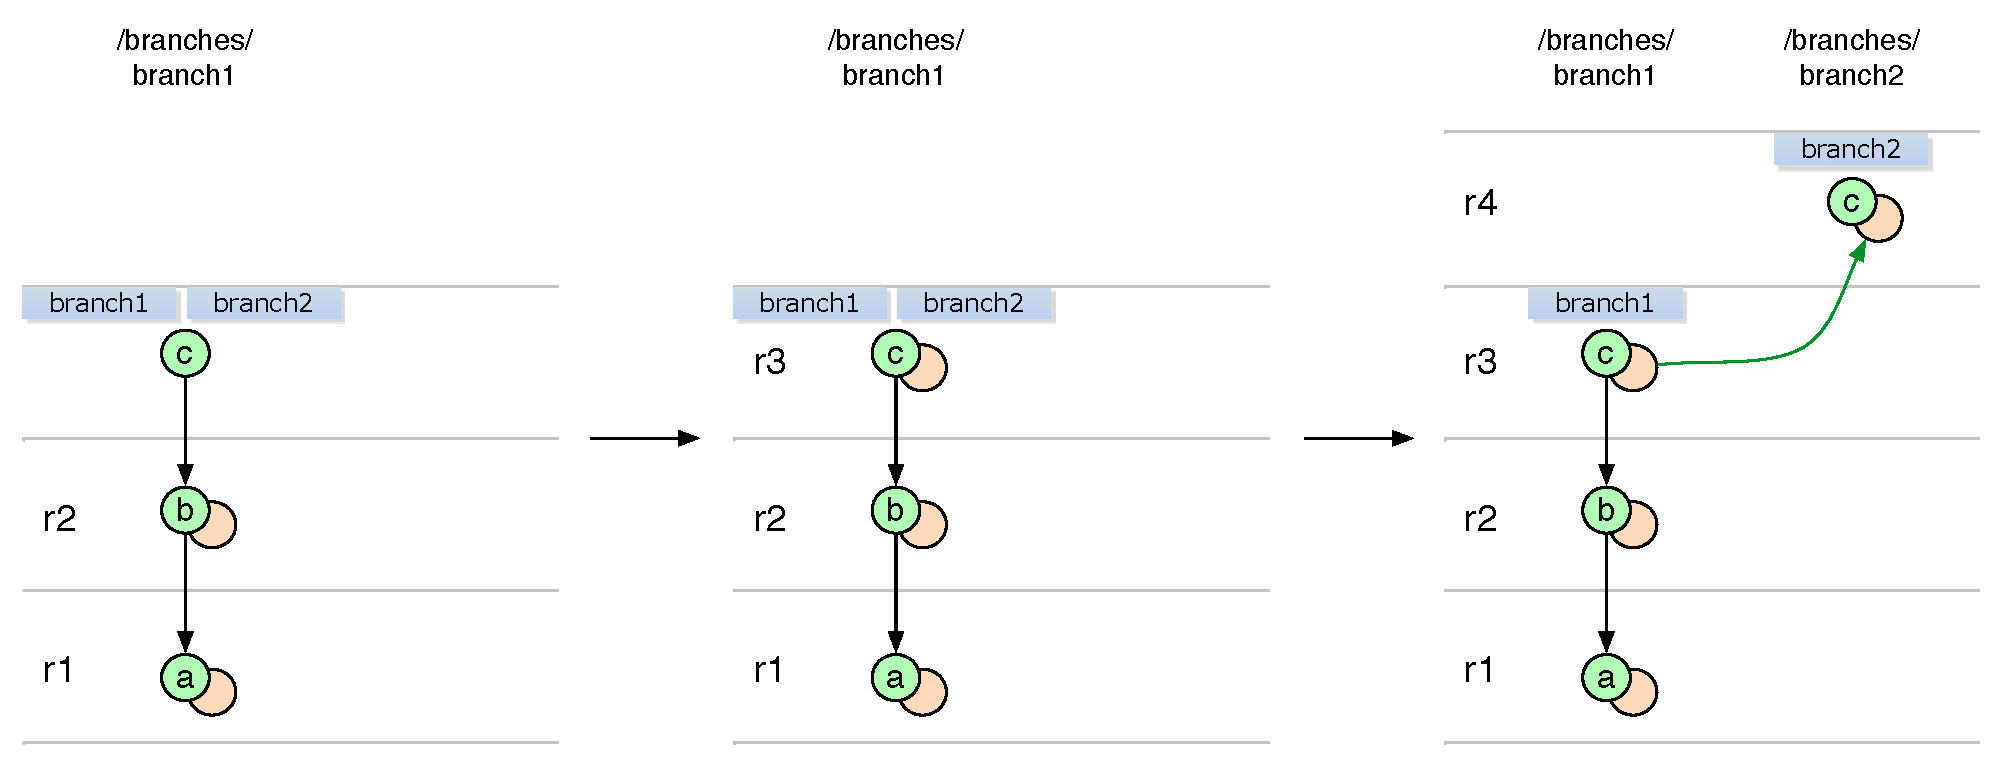
\includegraphics[width=\textwidth]{img/diagrams/ambiguous_svn_branch_git_to_svn.pdf}%
\captionof{figure}{Commit referenced by two branches being translated to Subversion two revisions: modification revision r3 and second branch creation revision r4.}
\label{ambiguous_svn_branch_git_to_svn}%
\end{center}

\subsubsection{Git Branch Deletion}

Deletion of the Git branch reference results in the deletion of the corresponding branches in Subversion repository, 
(diagram \ref{branch_deletion_git_to_svn}). Multiple Git branches could be removed at once and as a result Translator 
creates a single revision which removes every corresponding Subversion branch.
\begin{center}
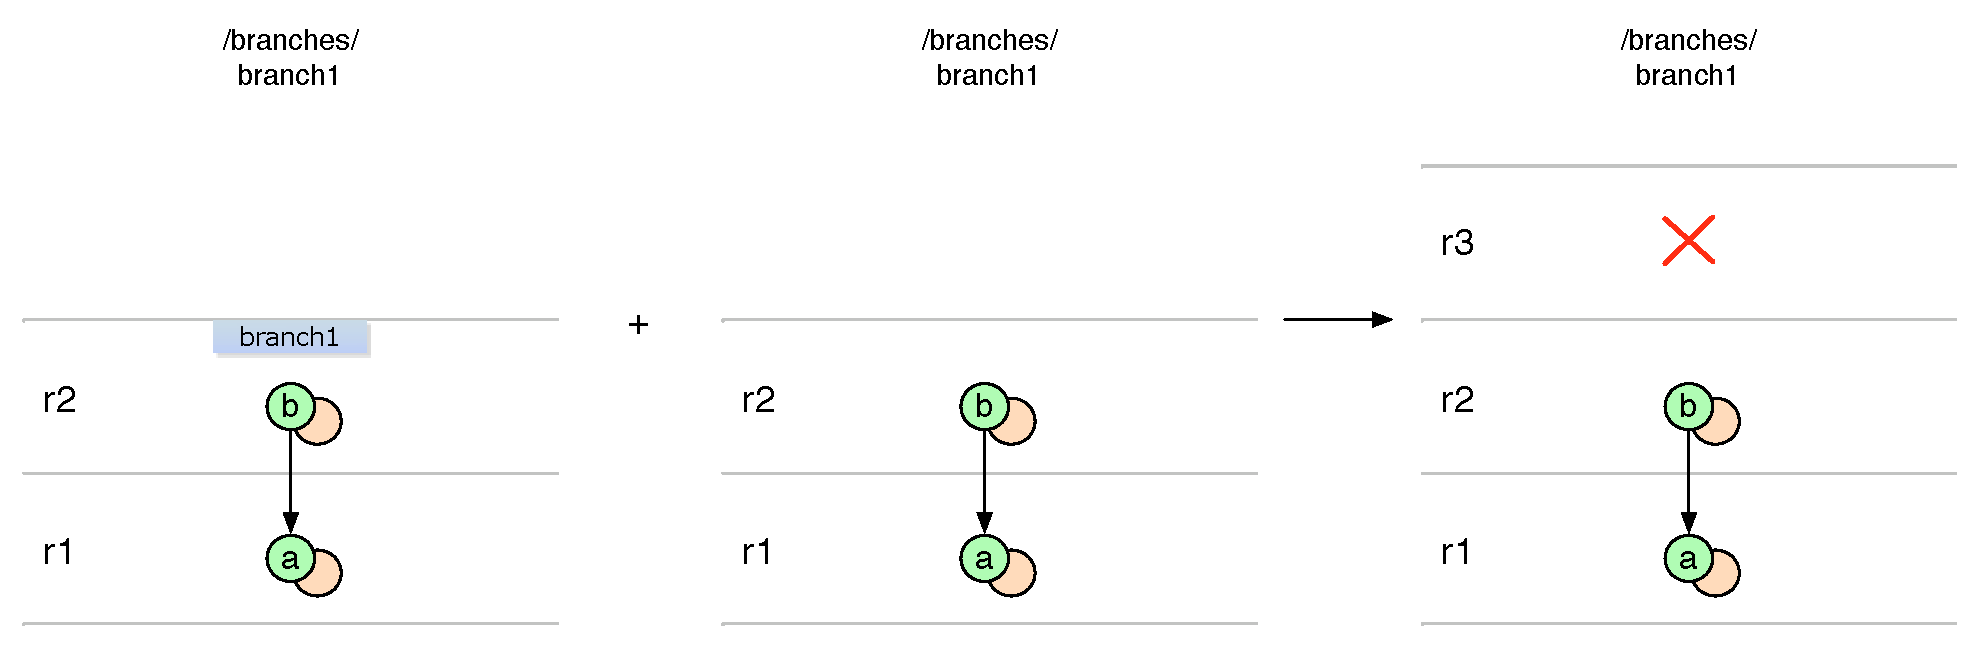
\includegraphics[width=\textwidth]{img/diagrams/branch_deletion_git_to_svn.pdf}%
\captionof{figure}{Deletion of Git branch being translated to Subversion branch removal.}
\label{branch_deletion_git_to_svn}%
\end{center}

\subsubsection{Git Branch Replacement}
Git user may reset any branch to any commit, and that kind of modification is translated as shown on the diagram \ref{branch_replacement_git_to_svn}.
\begin{center}
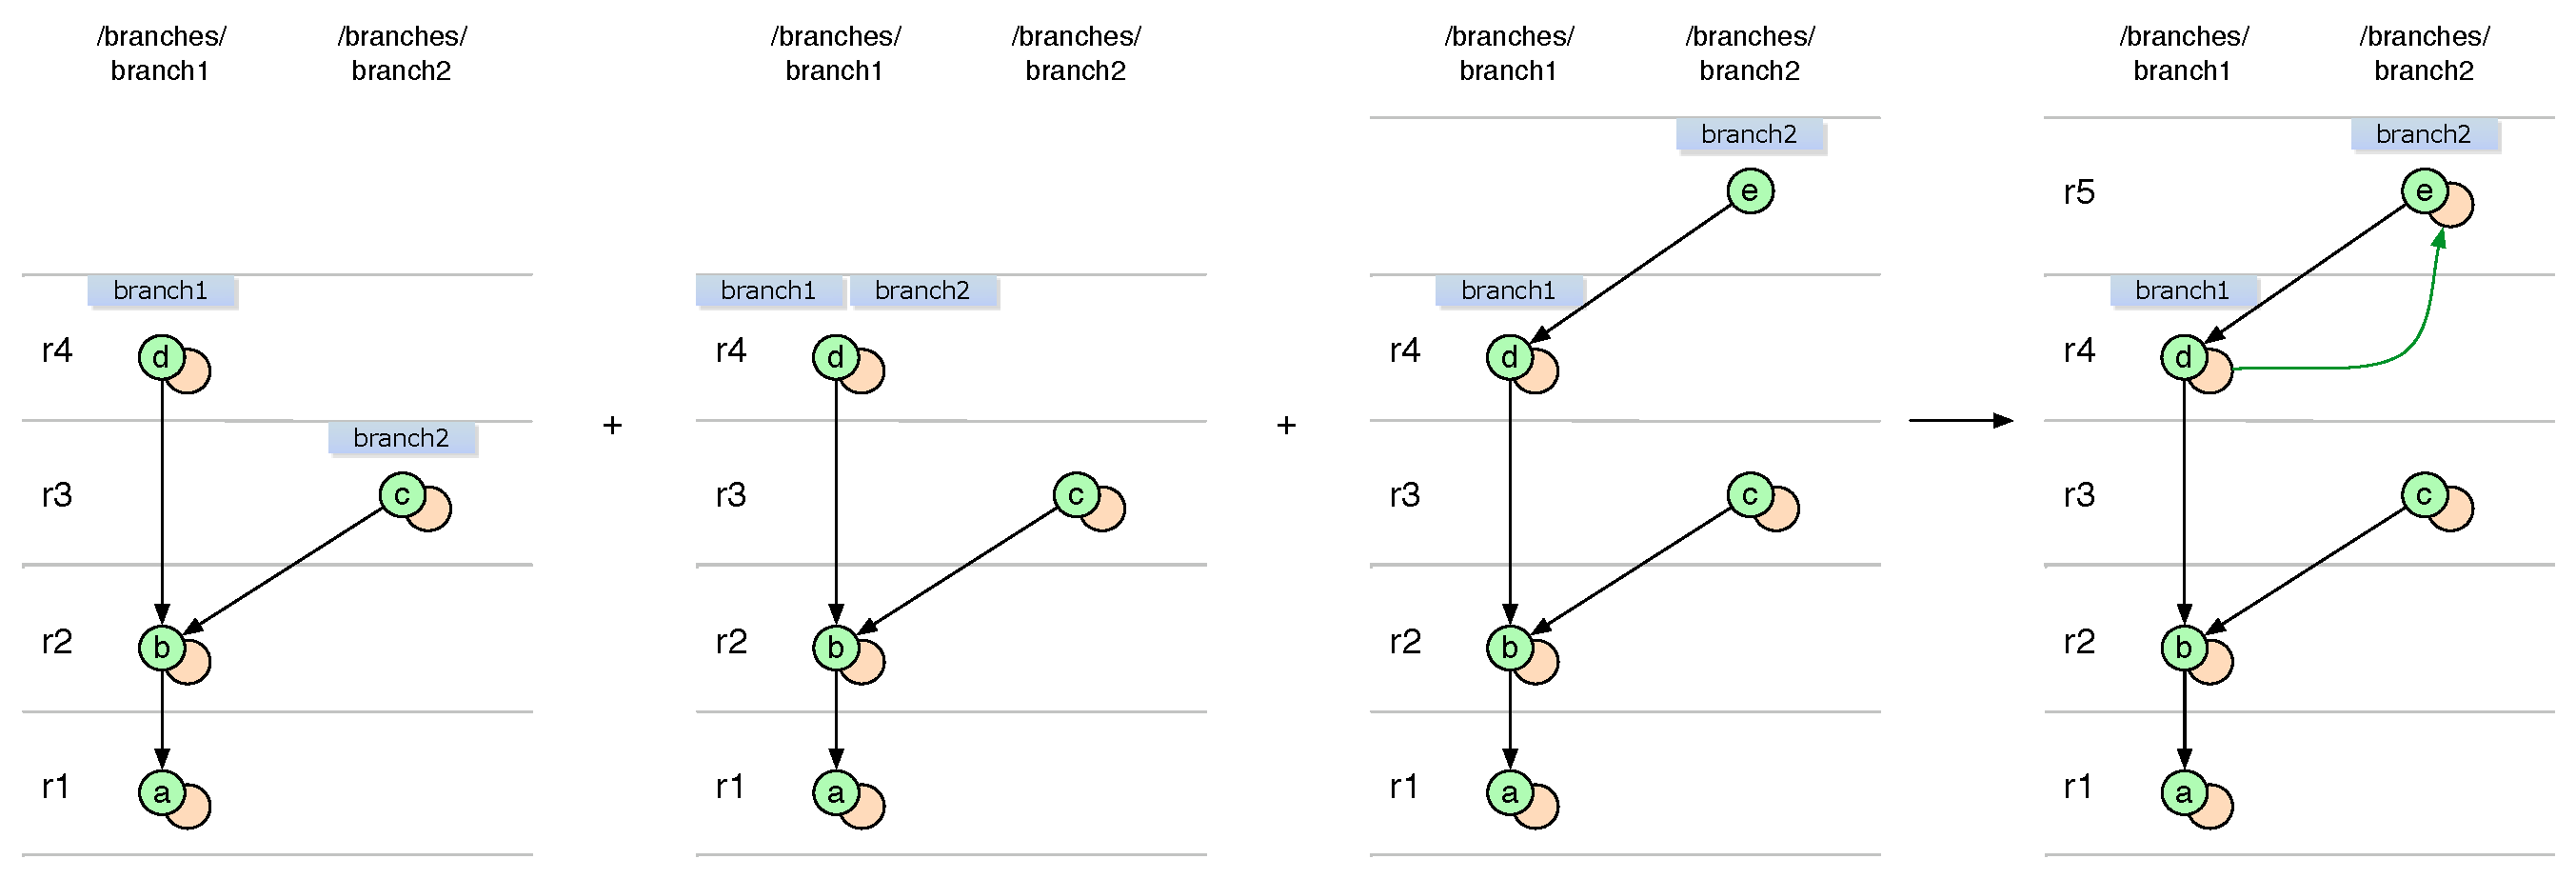
\includegraphics[width=\textwidth]{img/diagrams/branch_replacement_git_to_svn.pdf}%
\captionof{figure}{Replacement of Git branch being translated to replacement of Subversion branch.}
\label{branch_replacement_git_to_svn}%
\end{center}
